%!TEX root = main.tex
\chapter{Requirements}
\label{chap:requirements}
This chapter describes both functional and non-functional requirements the application should meet, in order to better support elaboration and implementation of the final application. Because of the time limitation, we did not expect to be able to implement every requirement, although all requirements were still a viable implementation in terms of the goals for this thesis. Since some of the requirements build on and is dependent on each other, the requirements described were used as a guide when implementing and not as a strict top-down list. 

\section{Functional Requirement}
\label{cha:funcreq}
The requirements detailed in this chapter are prioritized according to how important they are for the implementation, with a three step scale. 

\vspace{0.5cm}
\begin{itemize}
    \item[\textbf{H}]{High-priority requirements must be met by the application.} 
    \item[\textbf{M}]{Medium-priority requirements should be met by the application, but omission will severely limit the application.}
    \item[\textbf{L}]{Low-priority requirements is not vital to the application, but should be met if all high and medium requirements are met.}
\end{itemize}
\vspace{0.5cm}

For this thesis, a three step scale provides us with adequate data for decisions without sacrificing too much fidelity.
In addition to prioritizing the requirements based on importance, the requirements will also be prioritized according to how hard and time consuming they are to implement. These priorities will use the H-M-L scale as described below. 

\vspace{0.5cm}
\begin{itemize}
    \item[\textbf{H}]{High is something that will take more than 10 hours to implement.}
    \item[\textbf{M}]{Medium is something that will take between 5 and 10 hours to implement.}
    \item[\textbf{L}]{Low is something that will take less than 5 hours to implement.}
\end{itemize}
\vspace{0.5cm}
Annotating requirements with both importance and difficulty priorities provides a a way to perform a \emph{cost/benefit} analysis for each of the requirements. A cost/benefit analysis is a way of weighing the total value of benefits against the costs of implementing them\citep{cellini2010cost}.
\begin{equation}
Net Benefits = Total Benefits - Total Cost
\end{equation}
A requirement that is hard to implement fully, but is of little importance to the project as a whole could be dropped in benefit for a more important one (or a less difficult one), if time or costs involved are deemed to be to large.

\subsection{General Requirements}
The requirements in this section are the most general requirements for the PeacefulBanana application. These are related to the most common functionality users encounter during use, i.e. getting started with the application and logging in. All of the general requirements are set as \emph{H - Essential}, meaning they have a high importance, since all other requirements depend on these. 
\begin{itemize}
    \vspace{0.5cm}
	\item[\textbf{FR1}] Users must be able to register a new account. \\
        \textit{\small{An account is necessary in order to use the application. }}

        \begin{tabular}{| l | p{7cm} |}
            \hline
            \rowcolor[gray]{0.8}
            \textbf{Impact} & \textbf{Values} \\
            \hline
            Importance priority & \textbf{H} -- Essential \\
            Difficulty & \textbf{M} -- Implementation-time 5-10 hours\\
            \hline
        \end{tabular}
    \vspace{0.5cm}
    \item[\textbf{FR2}] Users must be able to log in \\
        \textit{\small{An active session is necessary in order to present user-specific data}}

        \begin{tabular}{| l | p{7cm} |}
            \hline
            \rowcolor[gray]{0.8}
            \textbf{Impact} & \textbf{Values} \\
            \hline
            Importance priority & \textbf{H} -- Essential \\
            Difficulty & \textbf{M} -- Implementation-time 5-10 hours \\
            \hline
        \end{tabular}
    \vspace{0.5cm}

    \item[\textbf{FR3}] Change password \\
        \textit{\small{As a [User] I want to [be able to change my password]}}

        \begin{tabular}{| l | p{7cm} |}
            \hline
            \rowcolor[gray]{0.8}
            \textbf{Impact} & \textbf{Values} \\
            \hline
            Importance priority & \textbf{H} -- Security wise, the ability to change password is very important\\
            Difficulty & \textbf{L} -- 5 hours \\
            \hline
        \end{tabular}
    \vspace{0.5cm}

    \item[\textbf{FR4}] Reset password \\
        \textit{\small{As a [User] I want to [be able to reset my password] if I forget it.}}

        \begin{tabular}{| l | p{7cm} |}
            \hline
            \rowcolor[gray]{0.8}
            \textbf{Impact} & \textbf{Values} \\
            \hline
            Importance priority & \textbf{H} -- If a user looses his password, a safe recovery procedure is important.\\
            Difficulty & \textbf{M} -- Reset-password functionality: 10 hours \\
            \hline
        \end{tabular}
    \vspace{0.5cm}

\subsection{GitHub Requirements}
The requirements in this section are related to what the application needs in order to collect satisfactory data from GitHub. This includes authorizing the application for use on a user's GitHub account and synchronization. 
    \item[\textbf{GR1}] GitHub account authorization\\
        \textit{\small{The application should be able to authorize the application with users GitHub account}}

        \begin{tabular}{| l | p{7cm} |}
            \hline
            \rowcolor[gray]{0.8}
            \textbf{Impact} & \textbf{Values} \\
            \hline
            Importance priority & \textbf{H} -- Essential as users need to allow the application to access data from their GitHub repositories\\
            Difficulty & \textbf{H} -- Could be very time consuming, 10-20 hours \\
            \hline
        \end{tabular}
    \vspace{0.5cm}

    \item[\textbf{GR2}] GitHub Synchronization\\
        \textit{\small{The application should be able to synchronize with GitHub whenever there is a new event or commit in one of the user's repositories.}}

        \begin{tabular}{| l | p{7cm} |}
            \hline
            \rowcolor[gray]{0.8}
            \textbf{Impact} & \textbf{Values} \\
            \hline
            Importance priority & \textbf{H} -- Essential. Synchronization is important in order to present the newest data to the users\\
            Difficulty & \textbf{H} -- Major functionality. 20-30 hours\\
            \hline
        \end{tabular}
    \vspace{0.5cm}

    \item[\textbf{GR3}] GitHub synchronization status \\
        \textit{\small{As a [User] I want to [be able to see my GitHub synchronization status] so I can see if I need to authenticate or if I haven't set a team.}}

        \begin{tabular}{| l | p{7cm} |}
            \hline
            \rowcolor[gray]{0.8}
            \textbf{Impact} & \textbf{Values} \\
            \hline
            Importance priority & \textbf{M} -- Moderately important, gives users feedback over their GitHub synchronization status and lets them know if any action is required.\\
            Difficulty & \textbf{L} -- 5 hours \\
            \hline
        \end{tabular}
    \vspace{0.5cm}

    \item[\textbf{GR4}] Force GitHub synchronization.\\
        \textit{\small{As a [User] I want to [be able to force a GitHub synchronization] so that I can ensure all the newest data are synchronized from GitHub.}}

        \begin{tabular}{| l | p{7cm} |}
            \hline
            \rowcolor[gray]{0.8}
            \textbf{Impact} & \textbf{Values} \\
            \hline
            Importance priority & \textbf{M} -- Changes on GitHub is automatically detected and updated by the application, but if this synchronization does not occur, allowing users to force it enables them to be sure that the newest data is included.\\
            Difficulty & \textbf{L} -- 5 hours \\
            \hline
        \end{tabular}
    \vspace{0.5cm}

\subsubsection{Team Requirements}
These requirements are concerned around connecting user and team specific features in the application with GitHub. This enables users to create a team consisting of users from their GitHub project, changing their roles on the PeacefulBanana application and joining other teams the user is a part of. The notion of a team is necessary in order to make use of the sharing of reflection notes, as mentioned in both scenarios in Section \ref{sec:scenarios}. 
    \item[\textbf{TR1}] Create a team\\
        \textit{\small{As a [User] I want to [create a team] so my fellow collaborators can join the team.}}

        \begin{tabular}{| l | p{8cm} |}
            \hline
            \rowcolor[gray]{0.8}
            \textbf{Impact} & \textbf{Values} \\
            \hline
            Importance priority & \textbf{H} -- Essential, a team need to be created for users to join it.\\
            Difficulty & \textbf{M} -- Moderately time consuming. 10 hours\\
            \hline
        \end{tabular}
    \vspace{0.5cm}

    \item[\textbf{TR2}] Join a team\\
        \textit{\small{As a [User] I want to [join a team from a list of available teams] so I can share and see shared reflection notes and other team relevant data.}}

        \begin{tabular}{| l | p{8cm} |}
            \hline
            \rowcolor[gray]{0.8}
            \textbf{Impact} & \textbf{Values} \\
            \hline
            Importance priority & \textbf{H} -- Essential, a team is required towards the collaborative and cooperative functions of the application, like reflection note sharing.\\
            Difficulty & \textbf{L} -- 5-10 hours\\
            \hline
        \end{tabular}
    \vspace{0.5cm}

    \item[\textbf{TR3}] Inspect my team\\
        \textit{\small{As a [User] I want to [inspect a team] so I see active members and their role in the team.}}

        \begin{tabular}{| l | p{8cm} |}
            \hline
            \rowcolor[gray]{0.8}
            \textbf{Impact} & \textbf{Values} \\
            \hline
            Importance priority & \textbf{H} -- Essential, users need to be able to see who is in their team in order to identify if someone is missing or an uninvited person is on their team.\\
            Difficulty & \textbf{L} -- Moderately time consuming. 5 hours\\
            \hline
        \end{tabular}
    \vspace{0.5cm}

    \item[\textbf{TR4}] Change team role\\
        \textit{\small{As a [Team Manager] I want to [be able to change the role of team members] so that I can ensure that the members have the correct user-role in the application.}}

        \begin{tabular}{| l | p{8cm} |}
            \hline
            \rowcolor[gray]{0.8}
            \textbf{Impact} & \textbf{Values} \\
            \hline
            Importance priority & \textbf{H} -- Essential, as only a team manager can access certain restricted functionality in the application.\\
            Difficulty & \textbf{M} -- Moderately time consuming. 10 hours\\
            \hline
        \end{tabular}
    \vspace{0.5cm}

\subsubsection{Milestone Requirements}
These requirements are related to both individual and collaborative use, as part of a preparation for the retrospective sessions mentioned in scenario 2, Section \ref{scenario2}. 
    \item[\textbf{MR1}] Active Milestones\\
        \textit{\small{As a [User] I want to [see what milestones are being worked on] so that I can see if the issues related to these milestones.}}

        \begin{tabular}{| l | p{7cm} |}
            \hline
            \rowcolor[gray]{0.8}
            \textbf{Impact} & \textbf{Values} \\
            \hline
            Importance priority & \textbf{M} -- Filtering milestones by their status allow users to see what milestones are unresolved and active, and find issues connected to these.\\
            Difficulty & \textbf{M} -- Moderately time consuming. 5-10 hours\\
            \hline
        \end{tabular}
    \vspace{0.5cm}

    \item[\textbf{MR2}] My closed issues\\
        \textit{\small{As a [User] I want to [see what issues have been closed] so that I inspect the issue and recollect how we solved the specific issue.}}

        \begin{tabular}{| l | p{7cm} |}
            \hline
            \rowcolor[gray]{0.8}
            \textbf{Impact} & \textbf{Values} \\
            \hline
            Importance priority & \textbf{M} -- Allowing revisiting of resolved issues gives users a chance to revisit and learn from previous mistakes or right-doings.\\
            Difficulty & \textbf{M} -- Moderately time consuming. 5-10 hours\\
            \hline
        \end{tabular}
    \vspace{0.5cm}

\subsection{Architectural Requirements}
The application is designed with a client-server architecture in mind, so the requirements here are divided to the specific parts of the architecture. In this case the client requirements concerns the application's graphical user interface and the server requirements concerns the application's back end functionality.
\begin{figure}[H]
\centering
    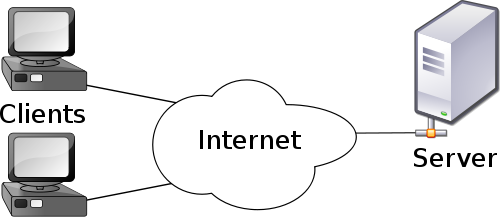
\includegraphics[width=0.8\textwidth]{client-server}
\caption{Client-server model \citep{clientServerModel}}
\label{csrlmodel}
\end{figure}

\subsubsection{Client Requirements}
These requirements are for the application graphical user interface and the functionality they need to have in order for them to perform the scenarios defined in section \ref{sec:scenarios}. Especially the core functionality featured in the \emph{Daily Reflection Note} and the sharing and inspection of these. 
    \item[\textbf{CR1}] Reflection Notes\\
        \textit{\small{As a [User] I want to [save my daily reflection notes] so I can review them at a later time.}}

        \begin{tabular}{| l | p{8cm} |}
            \hline
            \rowcolor[gray]{0.8}
            \textbf{Impact} & \textbf{Values} \\
            \hline
            Importance priority & \textbf{H} -- Essential, in order to support reflection, users need to be able to revisit experiences\\
            Difficulty & \textbf{M} -- Moderately time consuming. 5-10 hours\\
            \hline
        \end{tabular}
    \vspace{0.5cm}

    \item[\textbf{CR2}] Connect feelings \& mood with reflection notes\\
        \textit{\small{As a [User] I want to [connect my mood \& feelings to a reflection note] so I can revisit the feelings in the retrospective sessions.}}

        \begin{tabular}{| l | p{8cm} |}
            \hline
            \rowcolor[gray]{0.8}
            \textbf{Impact} & \textbf{Values} \\
            \hline
            Importance priority & \textbf{H} -- Essential, connecting a users mood to a specific experience help users revisit the experience\\
            Difficulty & \textbf{M} -- Moderately time consuming. 5-10 hours\\
            \hline
        \end{tabular}
    \vspace{0.5cm}

    \item[\textbf{CR3}] Tag-cloud\\
        \textit{\small{As a [User] I want to [see a tag cloud of my most active tags] so I can remember the situations I worked most on and reflect upon them.}}

        \begin{tabular}{| l | p{8cm} |}
            \hline
            \rowcolor[gray]{0.8}
            \textbf{Impact} & \textbf{Values} \\
            \hline
            Importance priority & \textbf{H} -- Essential, arranging the most active tags in a tag cloud will help users easily identify and separate the important situations from the less relevant ones\\
            Difficulty & \textbf{H} -- Highly time consuming. 10-15 hours\\
            \hline
        \end{tabular}
    \vspace{0.5cm}

    \item[\textbf{CR4}] Tag cloud: Personal vs Team\\
        \textit{\small{As a [User] I want to [compare my personal tag cloud with my team's tag cloud] so I can compare my issues with the teams trending issues}}

        \begin{tabular}{| l | p{8cm} |}
            \hline
            \rowcolor[gray]{0.8}
            \textbf{Impact} & \textbf{Values} \\
            \hline
            Importance priority & \textbf{H} -- Essential, comparing personal tagcloud with the team's help identify if the team's trending issues differ from yours\\
            Difficulty & \textbf{H} -- Highly time consuming. 10-15 hours\\
            \hline
        \end{tabular}
    \vspace{0.5cm}

    \item[\textbf{CR5}] Commit Impact\\
        \textit{\small{As a [User] I want to [see my commit impact] so I can compare my activity with the team's activity.}}

        \begin{tabular}{| l | p{8cm} |}
            \hline
            \rowcolor[gray]{0.8}
            \textbf{Impact} & \textbf{Values} \\
            \hline
            Importance priority & \textbf{M} -- Essential, gives users a general idea of who is contributing to the project\\
            Difficulty & \textbf{L} -- 5-10 hours\\
            \hline
        \end{tabular}
    \vspace{0.5cm}

    \item[\textbf{CR6}] Issues\\
        \textit{\small{As a [User] I want to [see my team's issues for the different milestones] so I can see the status of each milestones' issues.}}

        \begin{tabular}{| l | p{8cm} |}
            \hline
            \rowcolor[gray]{0.8}
            \textbf{Impact} & \textbf{Values} \\
            \hline
            Importance priority & \textbf{H} -- Essential, gives users a general idea of who is contributing to the project\\
            Difficulty & \textbf{M} -- Moderately time consuming. 10 hours\\
            \hline
        \end{tabular}
    \vspace{0.5cm}

    \item[\textbf{CR7}] Inspect Specific Issue\\
        \textit{\small{As a [User] I want to [inspect individual issues in a specific milestone] so I can see the status of the issue and what events that are related to this issue.}}

        \begin{tabular}{| l | p{8cm} |}
            \hline
            \rowcolor[gray]{0.8}
            \textbf{Impact} & \textbf{Values} \\
            \hline
            Importance priority & \textbf{H} -- Essential, gives users a general idea of who is contributing to the project\\
            Difficulty & \textbf{M} -- Moderately time consuming. 10 hours\\
            \hline
        \end{tabular}
    \vspace{0.5cm}

    \item[\textbf{CR8}] General Issues\\
        \textit{\small{As a [User] I want to [see my projects general issues] so I can see what is being worked on outside of particular milestones.}}

        \begin{tabular}{| l | p{8cm} |}
            \hline
            \rowcolor[gray]{0.8}
            \textbf{Impact} & \textbf{Values} \\
            \hline
            Importance priority & \textbf{M} -- Essential, gives users a general idea of who is contributing to the project\\
            Difficulty & \textbf{M} -- Moderately time consuming. 10-15 hours\\
            \hline
        \end{tabular}
    \vspace{0.5cm}

    \item[\textbf{CR9}] Share Reflection Notes\\
        \textit{\small{As a [User] I want to [share my reflection notes] so I can share my experiences with the team.}}

        \begin{tabular}{| l | p{8cm} |}
            \hline
            \rowcolor[gray]{0.8}
            \textbf{Impact} & \textbf{Values} \\
            \hline
            Importance priority & \textbf{H} -- Essential, users need to be able to share their notes with the team.\\
            Difficulty & \textbf{M} -- Moderately time consuming. 10 hours\\
            \hline
        \end{tabular}
    \vspace{0.5cm}

    \item[\textbf{CR10}] Sort Reflection Notes\\
        \textit{\small{As a [User] I want to [sort my reflection notes by 'Shared' status] so I can filter out my personal reflection notes from the team's.}}

        \begin{tabular}{| l | p{8cm} |}
            \hline
            \rowcolor[gray]{0.8}
            \textbf{Impact} & \textbf{Values} \\
            \hline
            Importance priority & \textbf{M} -- Moderately important, filtering enhances the user experience, but is not essential for the functionality of the application.\\
            Difficulty & \textbf{L} -- 5 hours\\
            \hline
        \end{tabular}
    \vspace{0.5cm}

    \item[\textbf{CR11}] Reflection Note reminder\\
        \textit{\small{As a [User] I want to [be reminded to do my daily reflection] so I always reflect and collect my experiences of that particular day.}}

        \begin{tabular}{| l | p{8cm} |}
            \hline
            \rowcolor[gray]{0.8}
            \textbf{Impact} & \textbf{Values} \\
            \hline
            Importance priority & \textbf{M} -- Essential, in order to support reflection, users need to be able to revisit experiences\\
            Difficulty & \textbf{L} -- 5 hours\\
            \hline
        \end{tabular}
    \vspace{0.5cm}

\subsubsection{Server Requirements}
These requirements are designed to ensure that the application works as intended in the scenarios in section \ref{sec:scenarios} and that the data is handled in a satisfactory manner. This includes a safely-encrypted persistent storage solution, MySQL and the required domain classes. 
    \item[\textbf{SR1}] Persistent Storage\\
        \textit{\small{Create MySQL database support for creating and performing actions on persistent databases by the application}}

        \begin{tabular}{| l | p{7cm} |}
            \hline
            \rowcolor[gray]{0.8}
            \textbf{Impact} & \textbf{Values} \\
            \hline
            Importance priority & \textbf{H} -- Essential, persistent storage is vital for the application to collect and store data\\
            Difficulty & \textbf{M} -- Moderately time consuming. 5-10 hours\\
            \hline
        \end{tabular}
    \vspace{0.5cm}

    \item[\textbf{SR2}] Databases\\
        \textit{\small{Create databases for different functionality: users, reflection notes, commits, milestones, repositories, etc}}

        \begin{tabular}{| l | p{7cm} |}
            \hline
            \rowcolor[gray]{0.8}
            \textbf{Impact} & \textbf{Values} \\
            \hline
            Importance priority & \textbf{H} -- Essential for functionality that requires synchronization with database\\
            Difficulty & \textbf{M} -- Moderately time-consuming. 8-10 hours\\
            \hline
        \end{tabular}
    \vspace{0.5cm}

    \item[\textbf{SR3}] Domain Classes\\
        \textit{\small{Create domain classes for the relation database}}

        \begin{tabular}{| l | p{7cm} |}
            \hline
            \rowcolor[gray]{0.8}
            \textbf{Impact} & \textbf{Values} \\
            \hline
            Importance priority & \textbf{H} -- Essential for all entities and their relations in the database \\
            Difficulty & \textbf{H} -- Could be very time consuming, 10+ hours \\
            \hline
        \end{tabular}
    \vspace{0.5cm}
\end{itemize}

%!TEX root = main.tex
%• Functional Requirements: Detail the requirements that you have to fulfill in order
%to complete the task.
\chapter{Non Functional Requirements}
\label{cha:nonfuncreq}
Non functional requirements of the application

\section{Usability}
According to Bass, Clements and Kazman, \emph{usability} is concerned about making the the tasks involved in the system as easy to accomplish as possible \cite[p.~90]{pensum}. Below we have identified the following use cases for assuring the usability of the application.

\begin{itemize}
    \item[\textbf{U1}] Support multiple resolutions \\
    \textit{\small{The users should be able to access the application on any device and screen size.}}
        
    \begin{tabular}{| l | p{7cm} |}
        \hline
        \rowcolor[gray]{0.8}
        \textbf{Portion of scenario} & \textbf{Values} \\
        \hline
        Source & Developer \\
        Stimulus & Make design responsive \\
        Artifact & System \\
        Environment & Run-time \\
        Response & Scale after resolution  \\
        Response measure & The application shall fit to the screensize \\
        \hline
    \end{tabular}

    \item[\textbf{U2}] Intuitiv design \\
    \textit{\small{The user interface must be easy to understand and not to create any confussion.}}
        
    \begin{tabular}{| l | p{7cm} |}
        \hline
        \rowcolor[gray]{0.8}
        \textbf{Portion of scenario} & \textbf{Values} \\
        \hline
        Source & Developer \\
        Stimulus & Make user interface easy to use \\
        Artifact & System \\
        Environment & User interface \\
        Response & Place buttons in a 'natural' matter. \\
        Response measure & Users will find the link they are looking for more than 95\% of the time. \\
        \hline
    \end{tabular}

    \item[\textbf{U3}] The application shall show hints whereever appropriate. \\
        \textit{\small{The user gets well-founded recommendations, tips or warnings during use, in order to increase confidence.}}
        
        \begin{tabular}{| l | p{7cm} |}
            \hline
            \rowcolor[gray]{0.8}
            \textbf{Portion of scenario} & \textbf{Values} \\
            \hline
            Source & End User \\
            Stimulus & User is uncertain on how the application is used, or what their next move can be \\
            Artifact & System \\
            Environment & Run-time \\
            Response & A message box with tips \\
            Response measure  & User can use the application without problem regarding to applitions usebility in \emph{1 hour}\\
            \hline
        \end{tabular}
\end{itemize}

\section{Availability}
According to someone availability is concerned about making the application as availible as possible

\begin{itemize}
    \item[\textbf{A1}] Uptime \\
    \textit{\small{The application shall be availible more than 90\% of the time.}}
        
    \begin{tabular}{| l | p{7cm} |}
        \hline
        \rowcolor[gray]{0.8}
        \textbf{Portion of scenario} & \textbf{Values} \\
        \hline
        Source & End User \\
        Stimulus & Accessing website \\
        Artifact & System \\
        Environment & Website \\
        Response & Show the user the website it desires. \\
        Response measure & Webserver will be working correctly more than 90\% of the time. \\
        \hline
    \end{tabular}

    \item[\textbf{A2}] Persistent storrage \\
    \textit{\small{When the system is rebooted it needs to restore to the same state as before.}}
        
    \begin{tabular}{| l | p{7cm} |}
        \hline
        \rowcolor[gray]{0.8}
        \textbf{Portion of scenario} & \textbf{Values} \\
        \hline
        Source & End User \\
        Stimulus & Accessing website \\
        Artifact & System \\
        Environment & Website \\
        Response & Show the user the website it desires. \\
        Response measure & After shutdown the application shall recover to the same state as before every time. \\
        \hline
    \end{tabular}
\end{itemize}

\section{Security}


\begin{itemize}
    \item[\textbf{S1}] Secure data storage \\
    \textit{\small{The application shall store sensitiv data secured.}}
        
    \begin{tabular}{| l | p{7cm} |}
        \hline
        \rowcolor[gray]{0.8}
        \textbf{Portion of scenario} & \textbf{Values} \\
        \hline
        Source & Developers \\
        Stimulus & Add security messures. \\
        Artifact & System \\
        Environment & Run time \\
        Response & Secure data  \\
        Response measure & After positioning the ships, the user is able to change these positions, one at a time. \\
        \hline
    \end{tabular}

    \item[\textbf{S2}] Authentication \\
    \textit{\small{The users shall be authenticated to view sensitiv data.}}
        
    \begin{tabular}{| l | p{7cm} |}
        \hline
        \rowcolor[gray]{0.8}
        \textbf{Portion of scenario} & \textbf{Values} \\
        \hline
        Source & End User \\
        Stimulus & Requesting to view sensitiv data. \\
        Artifact & System \\
        Environment & Run time \\
        Response & Check authentication \\
        Response measure & If authenticated show the appropriate data. \\
        \hline
    \end{tabular}

\end{itemize}